 
\graphicspath{{png/}}
\section{Результаты моделей}
Так как данные очень хорошо линейно разделимы, явные выбросы были удалены, все модели дают одинаковый результат с поразительной точностью 98-88\%. 
Ниже приведены результаты всех моделей. Сначала модели, реализованные вручную, затем из библиотеки.

\subsection{Метод k-ближайших соседей}
\subsubsection{kNN}
\begin{alltt}
Best params: {'knn__k': 5}
Best acc: 0.8883529397690296
Accuracy: 0.8903571428571428
Recall: 0.9036144578313253
Precision: 0.8817427385892116
\end{alltt}
\begin{center}
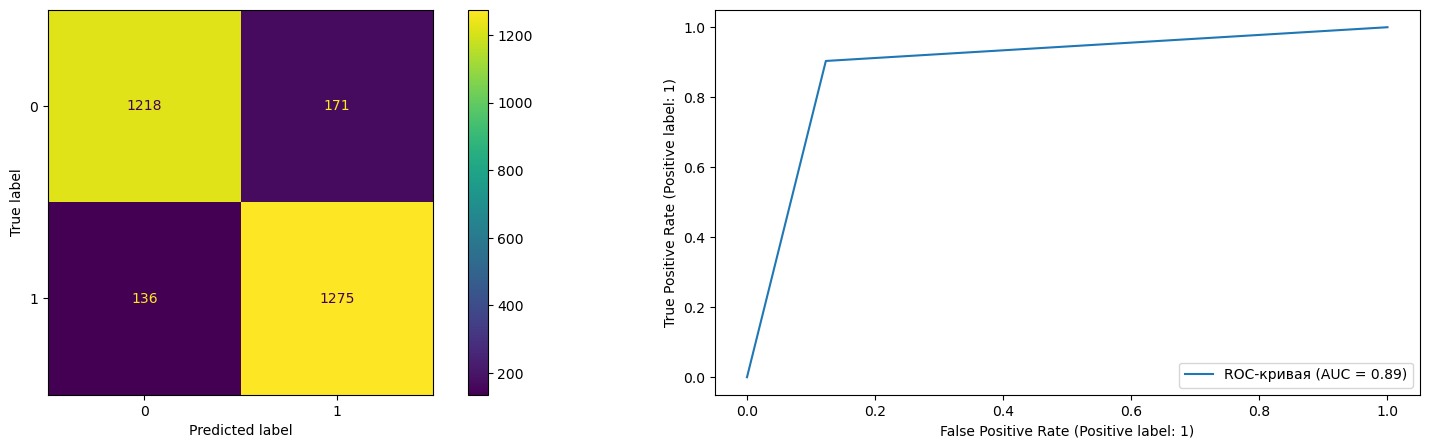
\includegraphics[width=\textwidth]{knn1}
\end{center}
\pagebreak

\subsubsection{sklearn.neighbors.KNeighborsClassifier}
\begin{alltt}
Best params: {'knn__n_neighbors': 5}
Best acc: 0.8883529397690296
Accuracy: 0.8903571428571428
Recall: 0.9036144578313253
Precision: 0.8817427385892116
\end{alltt}
\begin{center}
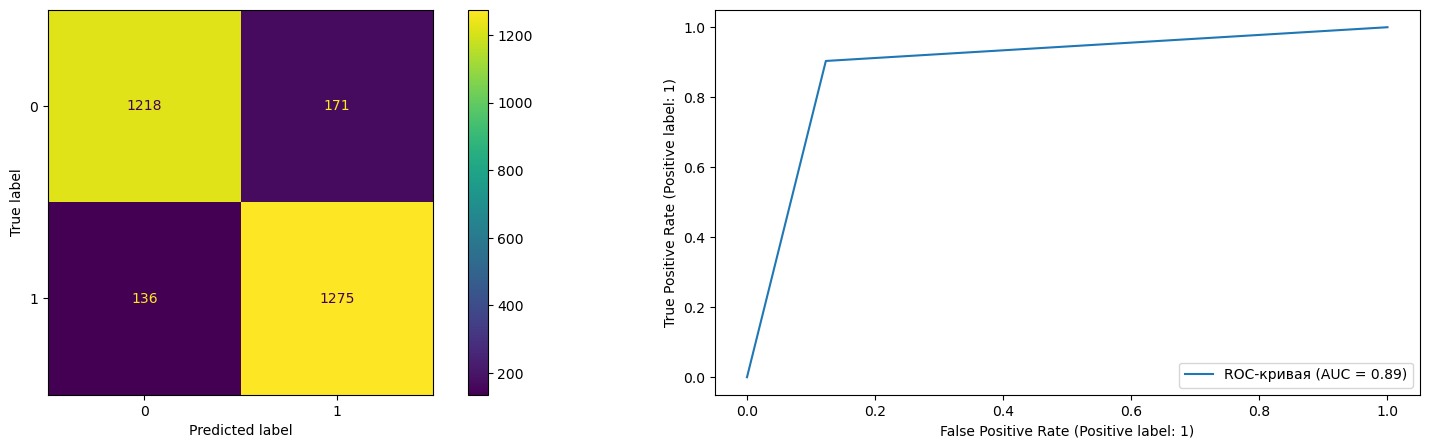
\includegraphics[width=\textwidth]{knn2}
\end{center}
\pagebreak

\subsection{Логистическая регрессия}
\subsubsection{LogisticRegression}
\begin{alltt}
Best params: {'logreg__SGD_step': 0.05, 'logreg__batch_size': 10, 'logreg__epoches': 4}
Best acc: 0.8060917262170613
Accuracy: 0.8003571428571429
Recall: 0.7973068745570517
Precision: 0.8047210300429185
\end{alltt}
\begin{center}
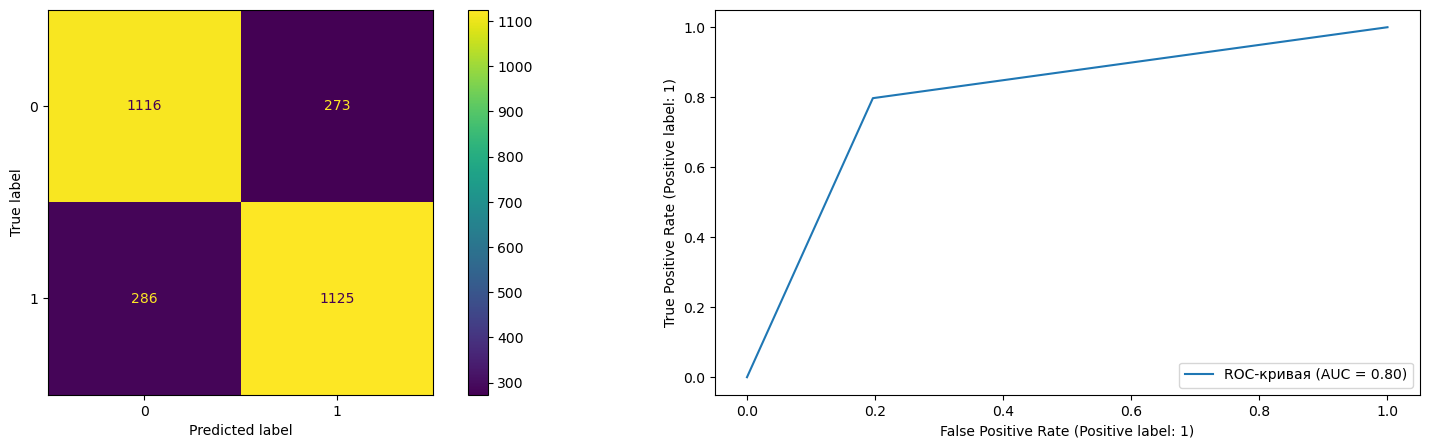
\includegraphics[width=\textwidth]{lr1}
\end{center}

\subsubsection{sklearn.linear\_model.LogisticRegression}
\begin{alltt}
Best params: {'logreg__max_iter': 1000, 'logreg__penalty': 'l2', 'logreg__solver': 'newton-cg'}
Best acc: 0.8034123572385632
Accuracy: 0.8025
Recall: 0.780297661233168
Precision: 0.8191964285714286
\end{alltt}
\begin{center}
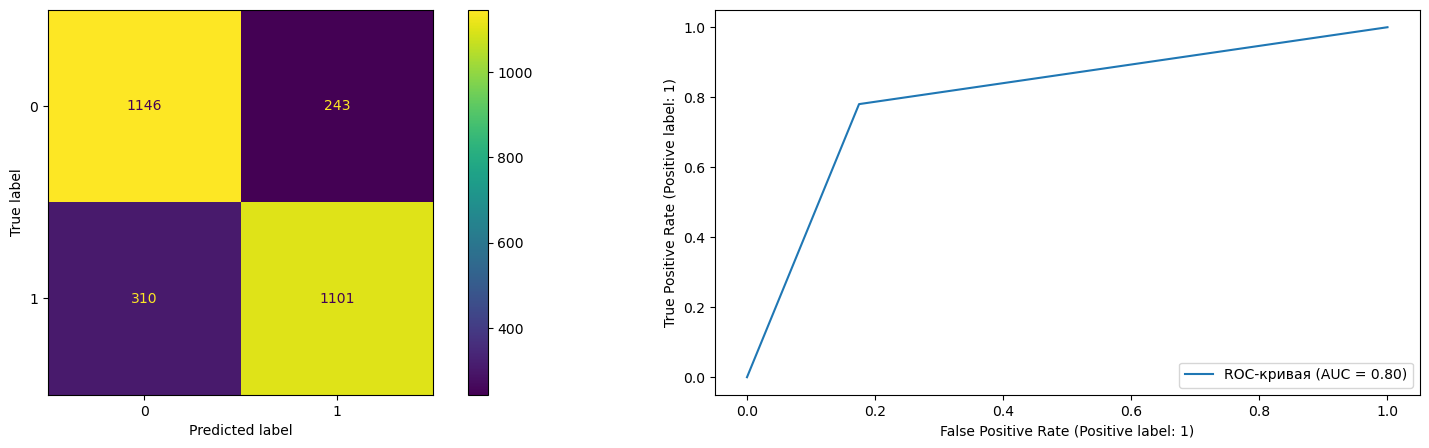
\includegraphics[width=\textwidth]{lr2}
\end{center}
\pagebreak

\subsection{Метод опорных векторов}
\subsubsection{SVM}
\begin{alltt}
Best params: {'SVM__SGD_step': 0.01, 'SVM__alpha': 0.0, 'SVM__batch_size': 10, 'SVM__epoches': 1}
Best acc: 0.8048408090346456
Accuracy: 0.8067857142857143
Recall: 0.8369950389794472
Precision: 0.7915549597855228
\end{alltt}
\begin{center}
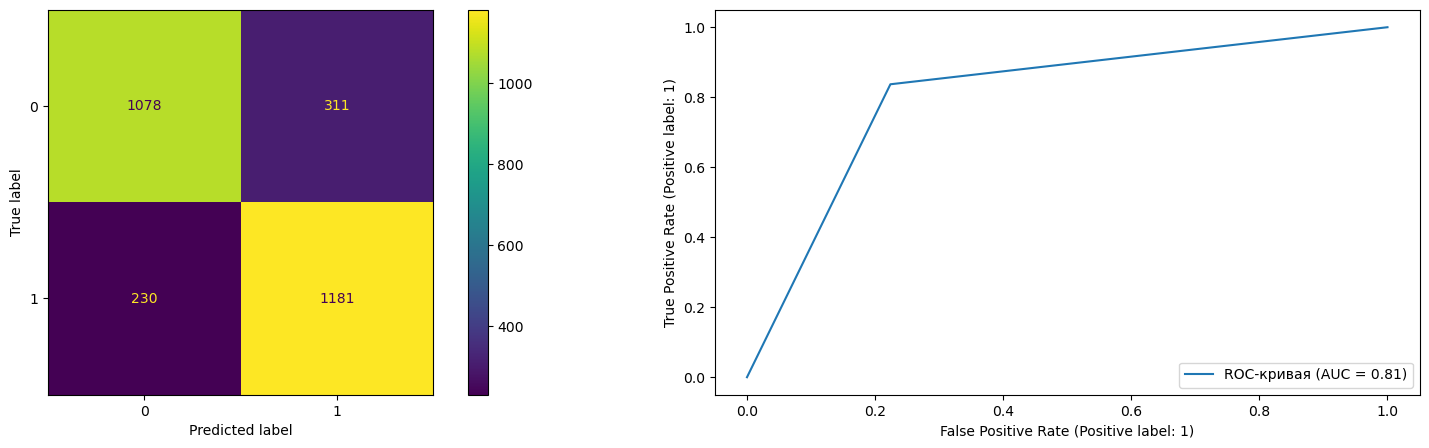
\includegraphics[width=\textwidth]{svm1}
\end{center}

\subsubsection{sklearn.svm.LinearSVC}
\begin{alltt}
Best params: {'svc__loss': 'hinge', 'svc__max_iter': 100000.0}
Best acc: 0.8068059720538505
Accuracy: 0.8085714285714286
Recall: 0.8199858256555634
Precision: 0.8040305767894371
\end{alltt}
\begin{center}
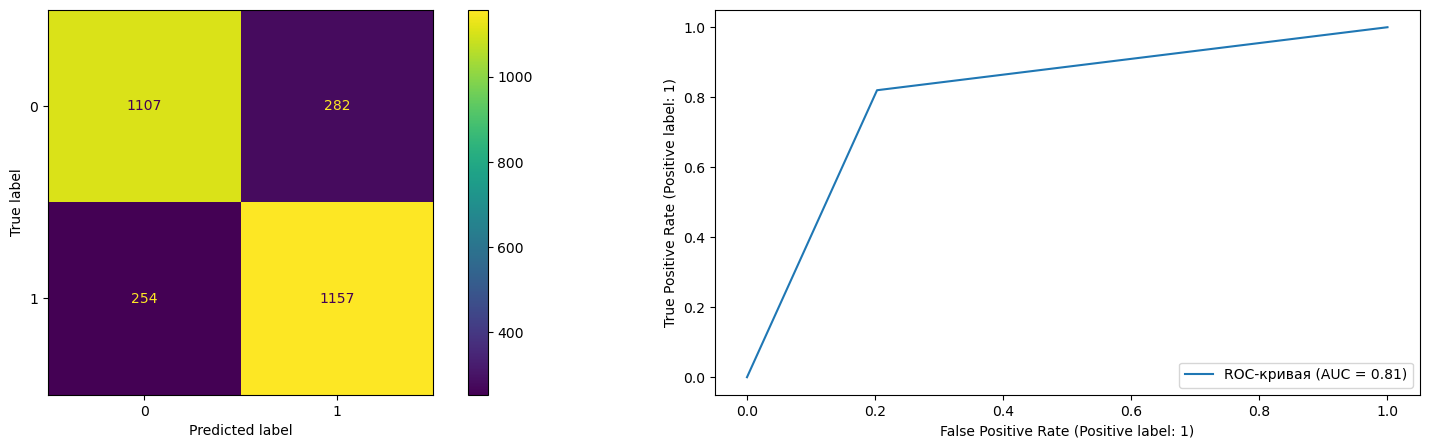
\includegraphics[width=\textwidth]{svm2}
\end{center}
\pagebreak

\subsection{Наивный байесовский классификатор}
\subsubsection{NaiveBayes}
\begin{alltt}
Accuracy: 0.8167857142857143
Recall: 0.8618001417434443
Precision: 0.7926988265971316
\end{alltt}
\begin{center}
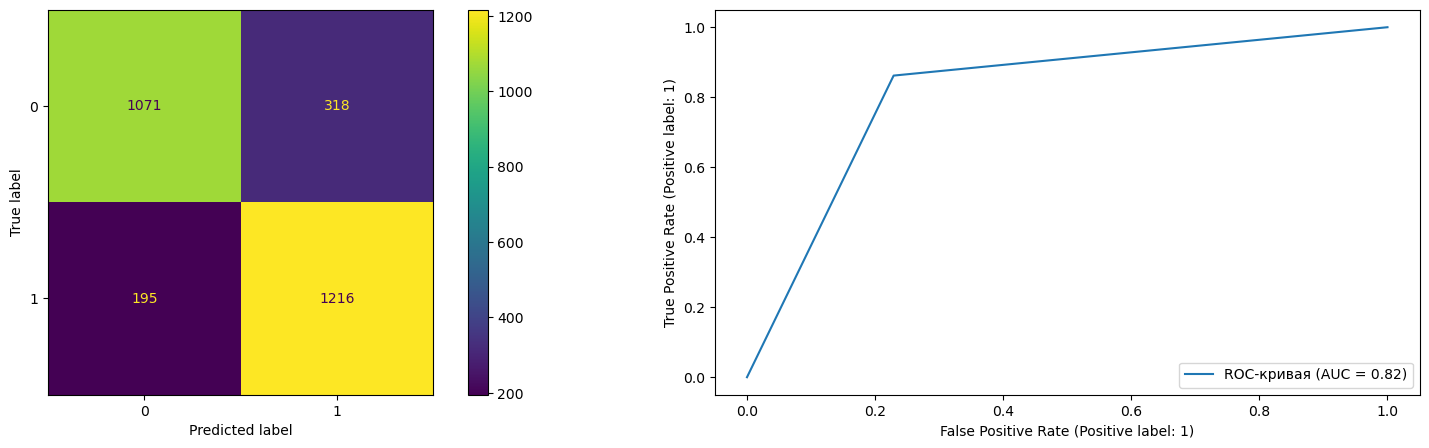
\includegraphics[width=\textwidth]{nb}
\end{center}

\subsubsection{sklearn.naive\_bayes.GaussianNB}
\begin{alltt}
Accuracy: 0.8367857142857142
Recall: 0.8476257973068746
Precision: 0.8317107093184979
\end{alltt}
\begin{center}
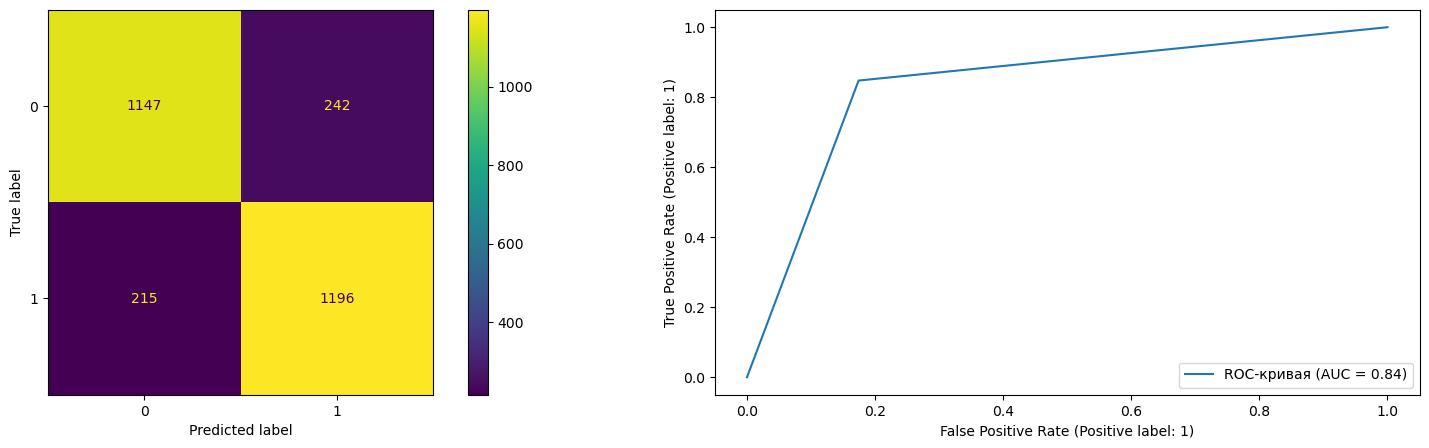
\includegraphics[width=\textwidth]{nb2}
\end{center}
\pagebreak
